\chapter{Framework}
\label{ch:methode}

In Kapitel \ref{ch:theorie} wurde das theoretisch-mathematische Modell beschrieben, mit welchem ein Bit geschrieben und wieder rekonstruiert werden kann. Um dieses Wissen nun praktisch nutzen zu können ist ein Framework notwenig in dem es zur Anwendung kommt. 

\section{Architektur}

Das von Shannon und Weaver entwickelte Sender-Empfänger-Modell \cite{shannon2001mathematical} kann herangezogen werden, um den schematischen Aufbau des Frameworks zu modellieren:

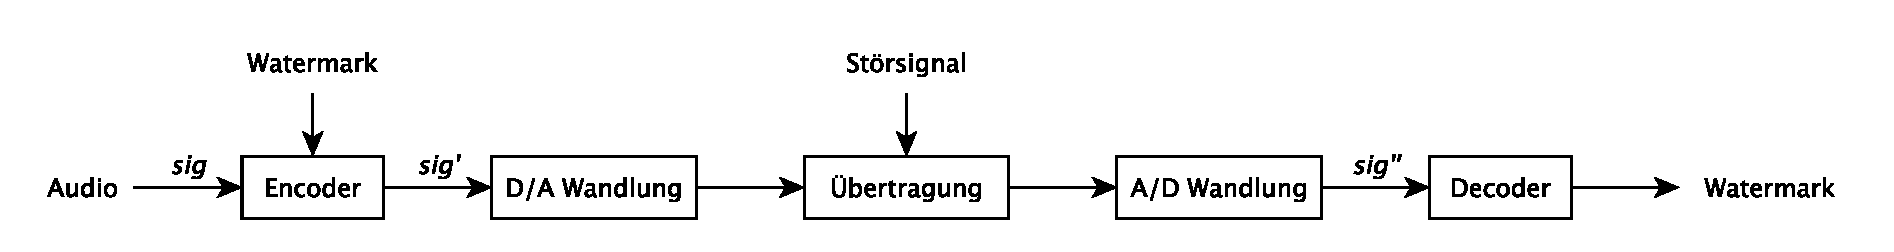
\includegraphics{figures/diagram-framework}


\begin{figure}[tb]
	\centering
	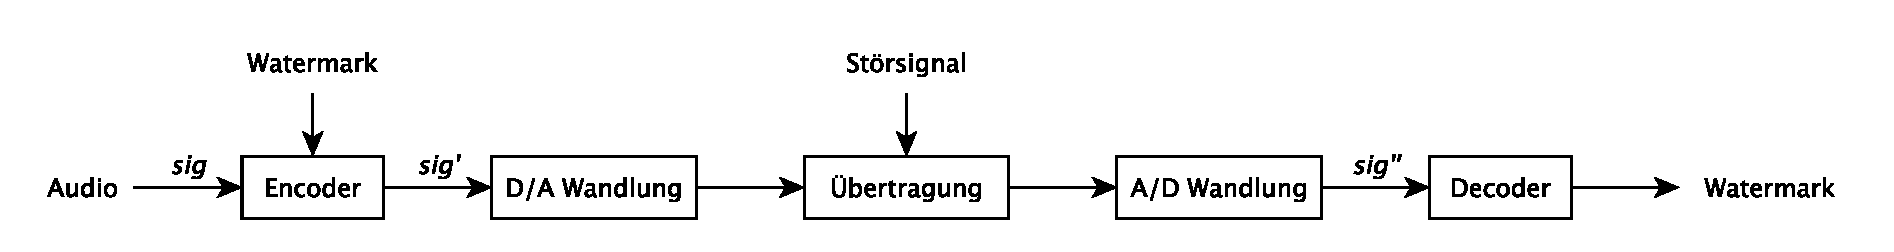
\includegraphics[width=0.7\textwidth]{figures/diagram-framework}
	\caption{Framework Übersicht}
	\label{fig:diagram-framework}
\end{figure}




Diagramme:

* kurzes über das ganze framework, hier am besten nur das watermark als ganzes einzeichnen
* watermark emedding
* watermark extraction

\section{Watermark Implantierung}
\label{sec:embedding}

\subsection{Synchronisations-Codes}

wozu sync codes ganz allgemein

\subsection{Fehlerkorrekturverfahren}
\label{sec:errorcorrection}

Error detection and correction

\subsubsection{BCH-Codes}

\cite{chang2012location} \cite{huang2002blind}

\subsubsection{RS-Codes}

\subsubsection{Turbo-Codes}

\subsection{Datenstrukturen und Protokoll}
\label{sec:protokoll}

\subsection{Qualitätskontrolle und ODG }
\label{sec:qualitaetskontrolle}

\subsubsection{Mean Opinion Score (MOS)}

\cite{??}

\subsubsection{Signal-Rauschabstand (SNR)} \index{Signal-Rauschabstand}

\subsubsection{Objective Difference Grade (ODG)} \index{Objective Difference Grade}

Eine kleine Evaluierung gängiger PEAQ Implementierungen findet sich in Anhang \ref{ch:peaq}.


\section{Watermark Extrahierung}
\label{sec:extraction}


\subsection{Resynchronisaton und Interpolation}

\subsection{Synchronisations-Code Erkennung}

\subsubsection{Autokorrelation und Barker-Codes} \index{Barker-Code}
\label{sec:barkercode}


vorteil der barker codes, autocorrelation

\subsection{Datenextrahierung}



